\documentclass{article}
\usepackage[english]{babel}
\usepackage[a4paper, total={6in, 10in}]{geometry}
\usepackage[T1]{fontenc}
\usepackage[utf8]{inputenc}
\usepackage{syntax}
\usepackage{url}
\usepackage{fancyvrb}
\usepackage{listings}
\usepackage{xcolor}
\usepackage{pgf}
\usepackage{tikz}
\usetikzlibrary{arrows,automata}
\usetikzlibrary{positioning}
\DefineVerbatimEnvironment{code}{Verbatim}{fontsize=\small}
\DefineVerbatimEnvironment{example}{Verbatim}{fontsize=\small}
\newcommand{\ignore}[1]{}
\definecolor{codegreen}{rgb}{0,0.6,0}
\definecolor{codegray}{rgb}{0.5,0.5,0.5}
\definecolor{codepurple}{rgb}{0.58,0,0.82}
\lstdefinestyle{mystyle}{
    commentstyle=\color{codegreen},
    keywordstyle=\color{magenta},
    numberstyle=\tiny\color{codegray},
    stringstyle=\color{codepurple},
    basicstyle=\ttfamily\footnotesize,
    breaklines=true,
    keepspaces=true,
    numbers=left,
    showspaces=false,
    showstringspaces=false,
    showtabs=false,
}
\lstset{style=mystyle}
\tikzset{
    state/.style={
           rectangle,
           rounded corners,
           draw=black, very thick,
           minimum height=2em,
           inner sep=2pt,
           text centered,
           },
}
\newenvironment{allintypewriter}{\ttfamily}{\par}

\title{Cruncher:\\
\large A Language for Handling Files and Folders}
\author{Jáder M. Camboim de Sá \\
        Department of Computer Science\\
        University of Brasília, Brazil \\
        jader.martins@ipea.gov.br}
\date{\today}

\begin{document}

\maketitle

\section{Introduction}
\label{sec:intro}
The Unix Shell is a general denomination for a command-line interpreter
(and a scripting language) that provides for users and systems admins an
interface to control the execution of operating system task's in Unix-like
environments \cite{negus2010linux}. This name comes from earlier times
when OS had this only interface covering the user interaction (like a shell
protecting the pearl). The Shell provides a way to create executable scripts,
execute programs, manage file-systems, compile code, and other general computer
manipulation tasks \cite{negus2010linux,blum2008linux}.

Although shells are very ancient computer technology, later being replaced by
graphical interfaces, many users (specially super-users) prefer this less
intuitive interface \cite{newham2005learning} for daily tasks. The \textit{sh}
is the precursor project and the default shell in many Unix distributions, but
many other shells were also developed with similar behavior but distinct
orientation. To cite a few, the most popular ones are \textit{bash}
\cite{bash}, \textit{zsh} \cite{zsh}, and \textit{fish} \cite{fish}.

Allied with the Shell, many external tools were developed to supply the needs
of Unix users \cite{negus2010linux}. Still, those were not integrated natively
in any of those shell scripting languages resulting in an inconsistent language
for file handling and operations. Tools like tar, sed, md5, etc, each has a
distinct parameter handling paradigm.

In modern \textbf{data processing}, a computing paradigm presented itself as a
suitable and intuitive way to describe massive computations and is adopted by
major frameworks like Hadoop \cite{white2012hadoop}, Spark
\cite{chambers2018spark}, and Kafka \cite{narkhede2017kafka}. The MapReduce is
a computational paradigm that decomposes computations in Maps and Reduction
operations. It has a clear and efficient computation model besides not being
so trivial to describe any computation in this paradigm
\cite{afrati2012vision}.

This paper proposes a language designed for \textbf{data processing} in shell,
specifically files, and folder processing in a standardized syntax, it
resembles the \textit{C} language but it adds a data type ``path'' and a
semantically consistent operation for external tools with an intuitive syntax.
It is organized in the following manner: Section \ref{sec:formal} describes the
formal grammar for Cruncher language, Section \ref{sec:semantics} presents the
semantics of principal keywords in the language, Section \ref{sec:error}
describes how it deals with errors, \ref{sec:proc} describes some procedures
applied by the scanner, \ref{sec:symtable} presents how it deals with
symbols , Section \ref{sec:syntax} presents how the Abstract Syntax Tree was
built, Sections \ref{sec:test} and \ref{sec:compiling} presents compiling and
testing the language, and finally, Section \ref{sec:conclusion} concludes the
paper.

\section{Formal Description}
\label{sec:formal}
In this section, we present the formal grammar for the \textit{Cruncher}
language, also we discuss notation and specification of the grammar. The
language extends the ANSI C \cite{kernighan2006c} by adding file handling
operations, incorporating external tools from the Unix shell in the same
syntax.

\paragraph{Notation Convention}
These notations convention are used for presenting syntax:

\begin{grammar}
\item $\epsilon$ - empty symbol.

\item ( \textit{pattern} )* - zero or more repetitions of the pattern.

\item ( \textit{pattern} )? - zero or one of the patterns.

\item \textit{symbol1} "..." \textit{symbol2} - a choice from symbol1 to symbol2.

\item <\textit{definition}> - definition for a statement.

\item "\textvisiblespace" - in some points, the space is made visible to
    emphasize his existence.
\end{grammar}

\subsection{Lexical Syntax}

\begin{grammar}
<translation-unit> ::= {<external-declaration>}*

<external-declaration> ::= <function-definition>
                         | <declaration>

<function-definition> ::= {<type-specifier>}* <declarator> {<declaration>}* <compound-statement>

<type-specifier> ::= "void"
\alt "char"
\alt "int"
\alt "long"
\alt "float"
\alt "path"

<constant-expression> ::= <conditional-expression>

<conditional-expression> ::= <logical-or-expression>
\alt <logical-or-expression> "?" <expression> ":" <conditional-expression>

<logical-or-expression> ::= <logical-and-expression>
\alt <logical-or-expression> "||" <logical-and-expression>

<logical-and-expression> ::= <inclusive-or-expression>
\alt <logical-and-expression> "&&" <inclusive-or-expression>

<equality-expression> ::= <relational-expression>
\alt <equality-expression> "==" <relational-expression>
\alt <equality-expression> "!=" <relational-expression>

<relational-expression> ::= <shift-expression>
\alt <relational-expression> "<" <shift-expression>
\alt <relational-expression> ">" <shift-expression>
\alt <relational-expression> "<=" <shift-expression>
\alt <relational-expression> ">=" <shift-expression>

<additive-expression> ::= <multiplicative-expression>
\alt <additive-expression> "+" <multiplicative-expression>
\alt <additive-expression> "-" <multiplicative-expression>

<multiplicative-expression> ::= <cast-expression>
\alt <multiplicative-expression> "*" <cast-expression>
\alt <multiplicative-expression> "/" <cast-expression>
\alt <multiplicative-expression> "\%" <cast-expression>

<primary-expression> ::= <identifier> | <constant> | <string> | ( <expression> )

<constant> ::= <integer-constant>
\alt <character-constant>
\alt <floating-constant>

<expression> ::= <assignment-expression> | <expression> , <assignment-expression>

<assignment-expression> ::= <conditional-expression>
\alt <unary-expression> <assignment-operator> <assignment-expression>

<assignment-operator> ::= "="

<type-name> ::= {<specifier-qualifier>}+ {<abstract-declarator>}?

<parameter-type-list> ::= <parameter-list>
                        | <parameter-list> , ...

<parameter-list> ::= <parameter-declaration>
                   | <parameter-list> , <parameter-declaration>

<parameter-declaration> ::= {<type-specifier>}+ <declarator>
                          | {<type-specifier>}+ <abstract-declarator>
                          | {<type-specifier>}+

<direct-abstract-declarator> ::=  ( <abstract-declarator> )
\alt {<direct-abstract-declarator>}? [ {<constant-expression>}? ]
\alt {<direct-abstract-declarator>}? ( {<parameter-type-list>}? )

<declaration> ::=  {<type-specifier>}+ {<init-declarator>}* ;

<init-declarator> ::= <declarator> | <declarator> = <initializer>

<initializer> ::= <assignment-expression> | { <initializer-list> } | { <initializer-list> , }

<initializer-list> ::= <initializer> | <initializer-list> , <initializer>

<compound-statement> ::= "{" {<declaration>}* {<statement>}* "}"

<statement> ::= <expression-statement>
\alt <compound-statement>
\alt <selection-statement>
\alt <iteration-statement>
\alt <jump-statement>
\alt <crunch-statement>

<expression-statement> ::= {<expression>}? ;

<selection-statement> ::= "if" "(" <expression> ")" <statement>
\alt "if" "(" <expression> ")" <statement> "else" <statement>

<iteration-statement> ::= "while" "(" <expression> ")" <statement>
\alt "for" "(" {<expression>}? ; {<expression>}? ; {<expression>}? ")" <statement>

<jump-statement> ::= "goto" <identifier>";"
\alt "continue;"
\alt "break;"
\alt "return" {<expression>}?";"

<crunch-statement> ::= "crunch" "(" <init-declarator> "\$"<crunch-op> <init-declarator> ")"

<crunch-op> ::= ">"|"*"|"+"|"&"|"!"|"@"
\end{grammar}

\subsection{Changes and Updates}
In the first version, the lexical syntax presented errors as complex structures
(e.g., context free grammars) were trying to be recognized at this step, but
those more complex structures should be recognized in the parser phase. The
second version corrected major problems. The new grammar is based on C, instead
of Haskell which was the previous base language, so many changes were applied.


\section{Semantics}
\label{sec:semantics}
The language's main feature is inspired in the MapReduce paradigm, which is a
popular design for data processing frameworks, so this language uses C
structured paradigm as his basis semantics. In this section we discuss the
semantics and exemplify the usage:

First, we begin exemplifying the <crunch> keyword:

\begin{verbatim}
/* replaces every occurrence of cat word in the files inplace.*/
int main() {
    path input = ."/home/jader/files/*.txt";
    path output = .".";
    crunch (input $!("s/cat/dog/g") output);
    return 0;
}


/*moves every content from those .txt files to a single .json file in json folder.*/
int main() {
    path input = ."/home/jader/files/*.txt";
    path output = _"/home/jader/json/file.json";
    crunch (input $> output);
    return 0;
}
\end{verbatim}

It has an input folder or file and an output folder or file, depending on the
kind of operation.  In Table \ref{tab:operations} some extra references for
additional symbols are shown, every operation has a single symbol. It replaces
the following Unix shell commands: \texttt{mv}, \texttt{rename}, \texttt{sed},
\texttt{tar} and \texttt{shaXsum}. As the language is in a premature stage,
only six crunch operations will be implemented in this phase, but later it
should support more than 32 shell operations.

The type of operation alternates the kind of matching between files, some have
a direct mapping, some perform an aggregation, and others both. For in-place
mapping, the output files can be implicitly defined by ``.'', if an aggregation
is performed, we must specify the  ``\_'' to be performed.

\begin{table}[ht]
    \centering
    \caption{Operations description}
    \label{tab:operations}
    \begin{tabular}{|c|c|l|} \hline
        Operation   & Symbol & Description\\ \hline
        Move        & >      & Move given files or directories \\
        Rename      & \&     & Renames given files or directories \\
        Edit        & !      & Stream editor operations \\
        Compression & @      & Compress files and/or directories using tar \\
        Hash        & *     & Calculates the hash \\
        Copy        & +     & Copy given files or directories \\ \hline
    \end{tabular}
\end{table}

\section{Error Handling}
\label{sec:error}
For the scanner phase, only local structures are recognized, so we use counters,
for line and column, to track locations of points with unrecognized tokens,
i.e., \texttt{line_count} and \texttt{line_count}, respectively. The
code below has exemplified this operation.

\begin{lstlisting}[language=C, caption=Example of code monitoring lines and columns.]
    %{
    int line_count = 1;
    int col_count = 1;
    %}
    EOL     \n
    ... /*some patterns*/
    %%
    EOL {
        line_count++;
        col_count = 1;
    }

    ... /*some patterns*/

    . {
        printf("Pattern unrecognized at line %d, column %d: %s\n",
                line_count, col_count+yyleng, yytext);
        return 1;
    }
\end{lstlisting}

If any other pattern is unrecognized it is captured by the `.', and reported.

\section{Procedures}
\label{sec:proc}
The Flex scanner provides many directives and variables to help in the scanning
process, four directives of this tool was used, \texttt{yyleng},
\texttt{yytext}, \texttt{yyin} and \texttt{yylineno}. The \texttt{yyleng}
returns the length of the current string recognized, the \texttt{yytext}
returns this string, the \texttt{yyin} read and return the file to be scanned.
All tokens are recognized and categorized by a macro \texttt{printLexeme}
defined in the following manner:

\begin{verbatim}
#define printLexeme(type) printf("A %s: \"%s\" at line %d\n",\
                                (type), yytext, line_count);
\end{verbatim}

There are two possible errors for scanning phase, (i) file ending in an
non terminated comment and (ii) a token not being recognized, generally given by
an special character in an non comment/string token. When an error occurs in the
scanning phase, this error is immediately reported and the scanning continues.

When an error occurs in the parsing phase (bad grammar construction), the
parser outputs the line and the kind of error and immediately terminates the
parsing.

The Bison is responsible for parsing, in a \texttt{.y} file we specify the
cruncher grammar which is later compiled in a parser to generate the abstract
syntax tree and the following intermediate code.

\section{Symbol Table}
\label{sec:symtable}
In Figure \ref{fig:symboltable} is shown an example of references in symbol
table, the symbol table is based on a hash map provided by \texttt{uthash} lib
\cite{hanson2013uthash} combined with the \texttt{utlist} by the same author,
initially a global table is created and for each function a local table is
defined with local definitions.

\begin{figure}[ht]
\label{fig:symboltable}
\centering
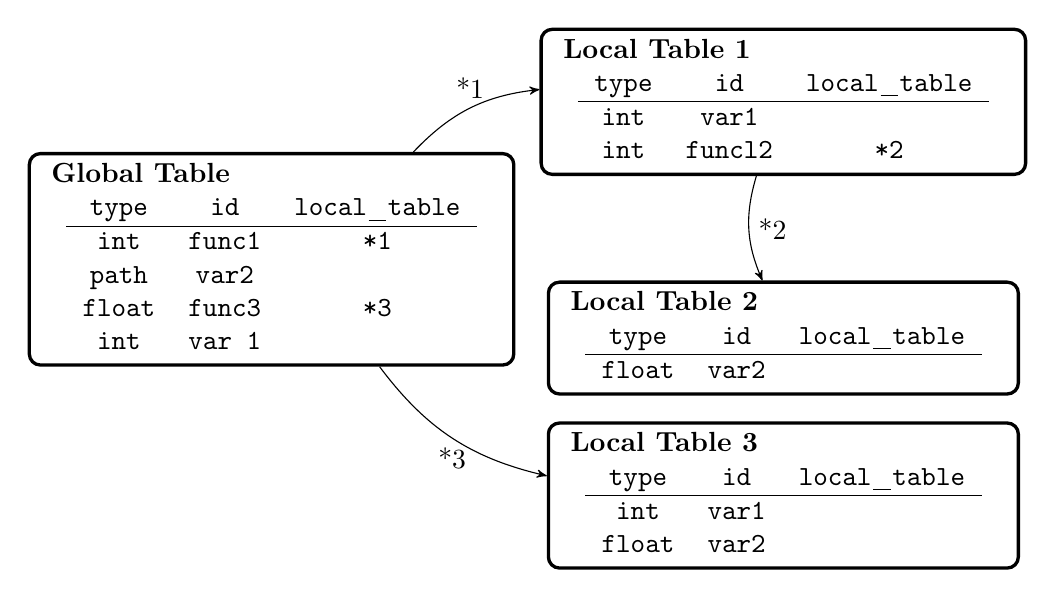
\begin{tikzpicture}[->,>=stealth']

 \node[state] (t0)
 {\begin{tabular}{l}
  \textbf{Global Table}\\
  \begin{allintypewriter}
  \begin{tabular}{ccc}
          type & id & local_table\\\hline
          int   & func1 & *1\\
          path & var2 & \\
          float & func3 & *3\\
          int   & var 1&
           \end{tabular}
  \end{allintypewriter}
 \end{tabular}
 };

 \node[state,
  yshift=2cm,
  right of=t0,
  node distance=6.5cm,
  anchor=center] (t1)
 {\begin{tabular}{l}
  \textbf{Local Table 1}\\
  \begin{allintypewriter}
  \begin{tabular}{ccc}
          type & id & local_table\\\hline
          int   & var1 & \\
          int   & funcl2 & *2
           \end{tabular}
  \end{allintypewriter}
 \end{tabular}
 };

 \node[state,
  below of=t1,
  node distance=3.0cm,
  anchor=center] (t2)
 {\begin{tabular}{l}
  \textbf{Local Table 2}\\
  \begin{allintypewriter}
  \begin{tabular}{ccc}
          type & id & local_table\\\hline
          float & var2 &
           \end{tabular}
  \end{allintypewriter}
 \end{tabular}
 };

 \node[state,
  yshift=1cm, 		% move 2cm in y
  below of=t2,
  node distance=3.0cm, 	% distance to QUERY
  anchor=center] (t3)
 {\begin{tabular}{l}
  \textbf{Local Table 3}\\
  \begin{allintypewriter}
  \begin{tabular}{ccc}
      type & id & local_table\\\hline
      int   & var1 \\
      float & var2
           \end{tabular}
  \end{allintypewriter}
 \end{tabular}
 };

 \path (t0) 	edge[bend left=20]  node[anchor=south,above]{*1} (t1)
 (t1)     	edge[bend right=20] node[anchor=south,right]{*2} (t2)
 (t0)     	edge[bend right=20] node[anchor=south,below]{*3} (t3);

\end{tikzpicture}
\caption{Example of symbol table.}
\end {figure}

So for a given identifier the symbol is searched in the possible stacked scope
until it reaches the end, returning if it exists or giving an error if the
symbol was not declared.

\section{Syntax Tree}%
\label{sec:syntax}
The syntax tree for the cruncher language is based on LALR, it was built using
structs with extra variables to handle the node values. The following code
presents this struct:

\begin{verbatim}
struct ast {
    int nodetype;
    struct ast *l;
    struct ast *r;
    char dtype;
    char *addr;
    union {
        char *str_;
        float float_;
        int int_;
        char char_;
    } value;
};
\end{verbatim}

The grammar is constructed with a binary tree, if a single rule needs more than
two nodes it expands left-recursive in nodes. For each node, if it is a
variable its type is set in dtype variable, if it is a crunch operation its
arguments are stored in addr.

\section{Semantic Analysis}
After the abstract tree was built in the semantic analysis are verified if the
types are adequate to applied operations and if some type conversion should be
executed.

In the node assignment arithmetic or booleand operations, the tree search every
operand if it matches the expected type, if not it tries to convert to the
expected type, if is not possible (e.g. string to float) it return an error.
In the case when operations are applied under an id, we search for the id type
in the symbol table to perform the same operation as above.

There are two kinds of type conversion, between numerical types (e.g. bool,
float, int) and between alphanumerical (e.g. char, string, path). The numerical
type type we convert bool to int by his binary representation (e.g. 0, 1), for
the opposite conversion we check if the integer is positive for true or
zero/negative for false. The float to int is just truncated to the upper
integer, the opposite conversion just represents it as in IEEE 754
\cite{ieee754}. By this process we can convert bool to float or float to bool
as explained above.

The alphanumerical types has a more complicated conversion, char can be
converted to string directly, but string only can be converted when the string
has size 1.  The path type can also be directly converted to string, but string
to be converted to path should start with a dot (.) or an underline (_), and
also it should be well formatted path. Additionally, char can be converted to
integer with his bits representation directly as a cardinal ascii, not a
literal interpretation.

The semantic step also checks if there is a \texttt{main} function and if every
invoked ID is present in the symbol table. If it is a function being declared
it can't overwrite a previously declared function, different from variables,
which can be overwriten. The function parameters are passed by copy through a
stack.

\section{Intermediate Code}
In the last step of the compiling procedure, the cruncher compiler generates a
three address code (TAC) based on the type checked abstract syntax tree (AST)
obtained from the previous step.  Then, the TAC, base on Aho \textit{et al.}
\cite{aho1986compilers}, is constructed by performing depth-first-search on the
AST, an for each node (depending on the type of node) a sequence of
instructions is appended to the final code. After that it can be interpreted in
the TAC Interpreter \cite{santos2020tac}.

Initially, it starts with an empty string using the UTstring lib, and at each
node value an instruction is appended to the code string. There are four types
of instructions being appended, gen0, gen1, gen2, and gen3, as explained in
\cite{aho1986compilers}. Each generated instruction has 0-3 extra parameters,
depending on the instruction nature. After the entire tree was traveled, the
final code is printed to a file ``\texttt{output.tac}''.

\section{Test files}
\label{sec:test}
There are two files for valid code examples and two for invalid codes. The
valid ones have the \texttt{test-valid} prefix, and the invalid,
\texttt{test-invalid} prefix.

\section{Compiling and Running}%
\label{sec:compiling}
This project provides a Makefile for compiling and testing, to compile run the
following commands in terminal:
\begin{verbatim}
    $ make lang
    $ make
\end{verbatim}

Then to run the test files use:
\begin{verbatim}
    $ make test
\end{verbatim}

Now you can run Cruncher with:
\begin{verbatim}
    $ ./bin/cruncher_lang file.cr
\end{verbatim}

\section{Conclusion}
\label{sec:conclusion}
The language presented in this paper aims to achieve a clear and consistent
syntax for files and folders handling, replacing the usual shell scripting that
requires external tools to made common operations that should be native in the
language. It is done by applying the functional scheme from Haskell allied to
the MapReduce paradigm. With two additional structures, it captures major
operations done in the Unix terminal using a minimal and intuitive syntax.

\bibliographystyle{alpha}
\bibliography{ref.bib}

\end{document}
